\RequirePackage{luatex85}
\documentclass[border=6pt]{standalone}
\usepackage{tikz}
\usepackage[compat=1.1.0]{tikz-feynman}
\usepackage{amsmath}
\usetikzlibrary{decorations.pathmorphing,decorations.markings,arrows.meta,patterns}

\begin{document}
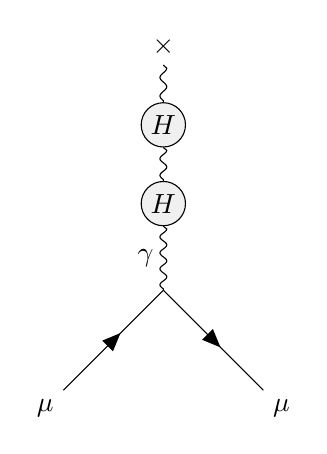
\begin{tikzpicture}
\begin{feynman}
  \vertex at (0, 3.6) (top) {\(\times\)};
  \vertex [circle, draw, fill=gray!12, minimum size=16pt, inner sep=0pt] at (0, 2.6) (H1) {\(H\)};
  \vertex [circle, draw, fill=gray!12, minimum size=16pt, inner sep=0pt] at (0, 1.6) (H2) {\(H\)};
  \vertex at (0, 0.5) (vtx);
  \vertex at (-1.5, -1.0) (lmu) {\(\mu\)};
  \vertex at (1.5, -1.0) (rmu) {\(\mu\)};
  \diagram* {
    (lmu) -- [fermion] (vtx) -- [fermion] (rmu),
    (vtx) -- [photon, edge label=\(\gamma\)] (H2),
    (H2) -- [photon] (H1),
    (H1) -- [photon] (top),
  };
\end{feynman}
\end{tikzpicture}
\end{document}
